\documentclass{standalone}
%\usepackage{fullpage}
\usepackage{tikz}

\usetikzlibrary{positioning}
%\usetikzlibrary{shapes.multipart}

\tikzstyle{rootClass}=[rectangle,black,draw, fill=orange!30, text width=8 cm]
\tikzstyle{essentialClass}=[rectangle,black,draw, fill=green!30, text width=8 cm]
\tikzstyle{exampleClass}=[rectangle,black,draw, fill=red!30, text width=8 cm]

\tikzstyle{inheritedFrom}=[->,black, line width=2]
\tikzstyle{instantiatedIn}=[-,black, line width=2] 
%Note that A instantiatedIn B relationship reduces flexibility as the 
%children of A cannot be known to B now.

\newcommand{\nodeTextWidthRatio}{0.95}
\newcommand{\method}[1]{\textbf{\texttt{#1}}}
\newcommand{\desc}[1]{\ \ \ #1}
\newcommand{\className}[1]{\large \textbf{#1}}
\newcommand{\data}[1]{\textbf{\texttt{#1}}}

\def\showExampleClasses{1}
\def\showEssentialClasses{1}
%Note that you can't have showExampleClasses=1 with showEssentialClasses=0
%as the former refer to the later and this will cause error.

\begin{document}

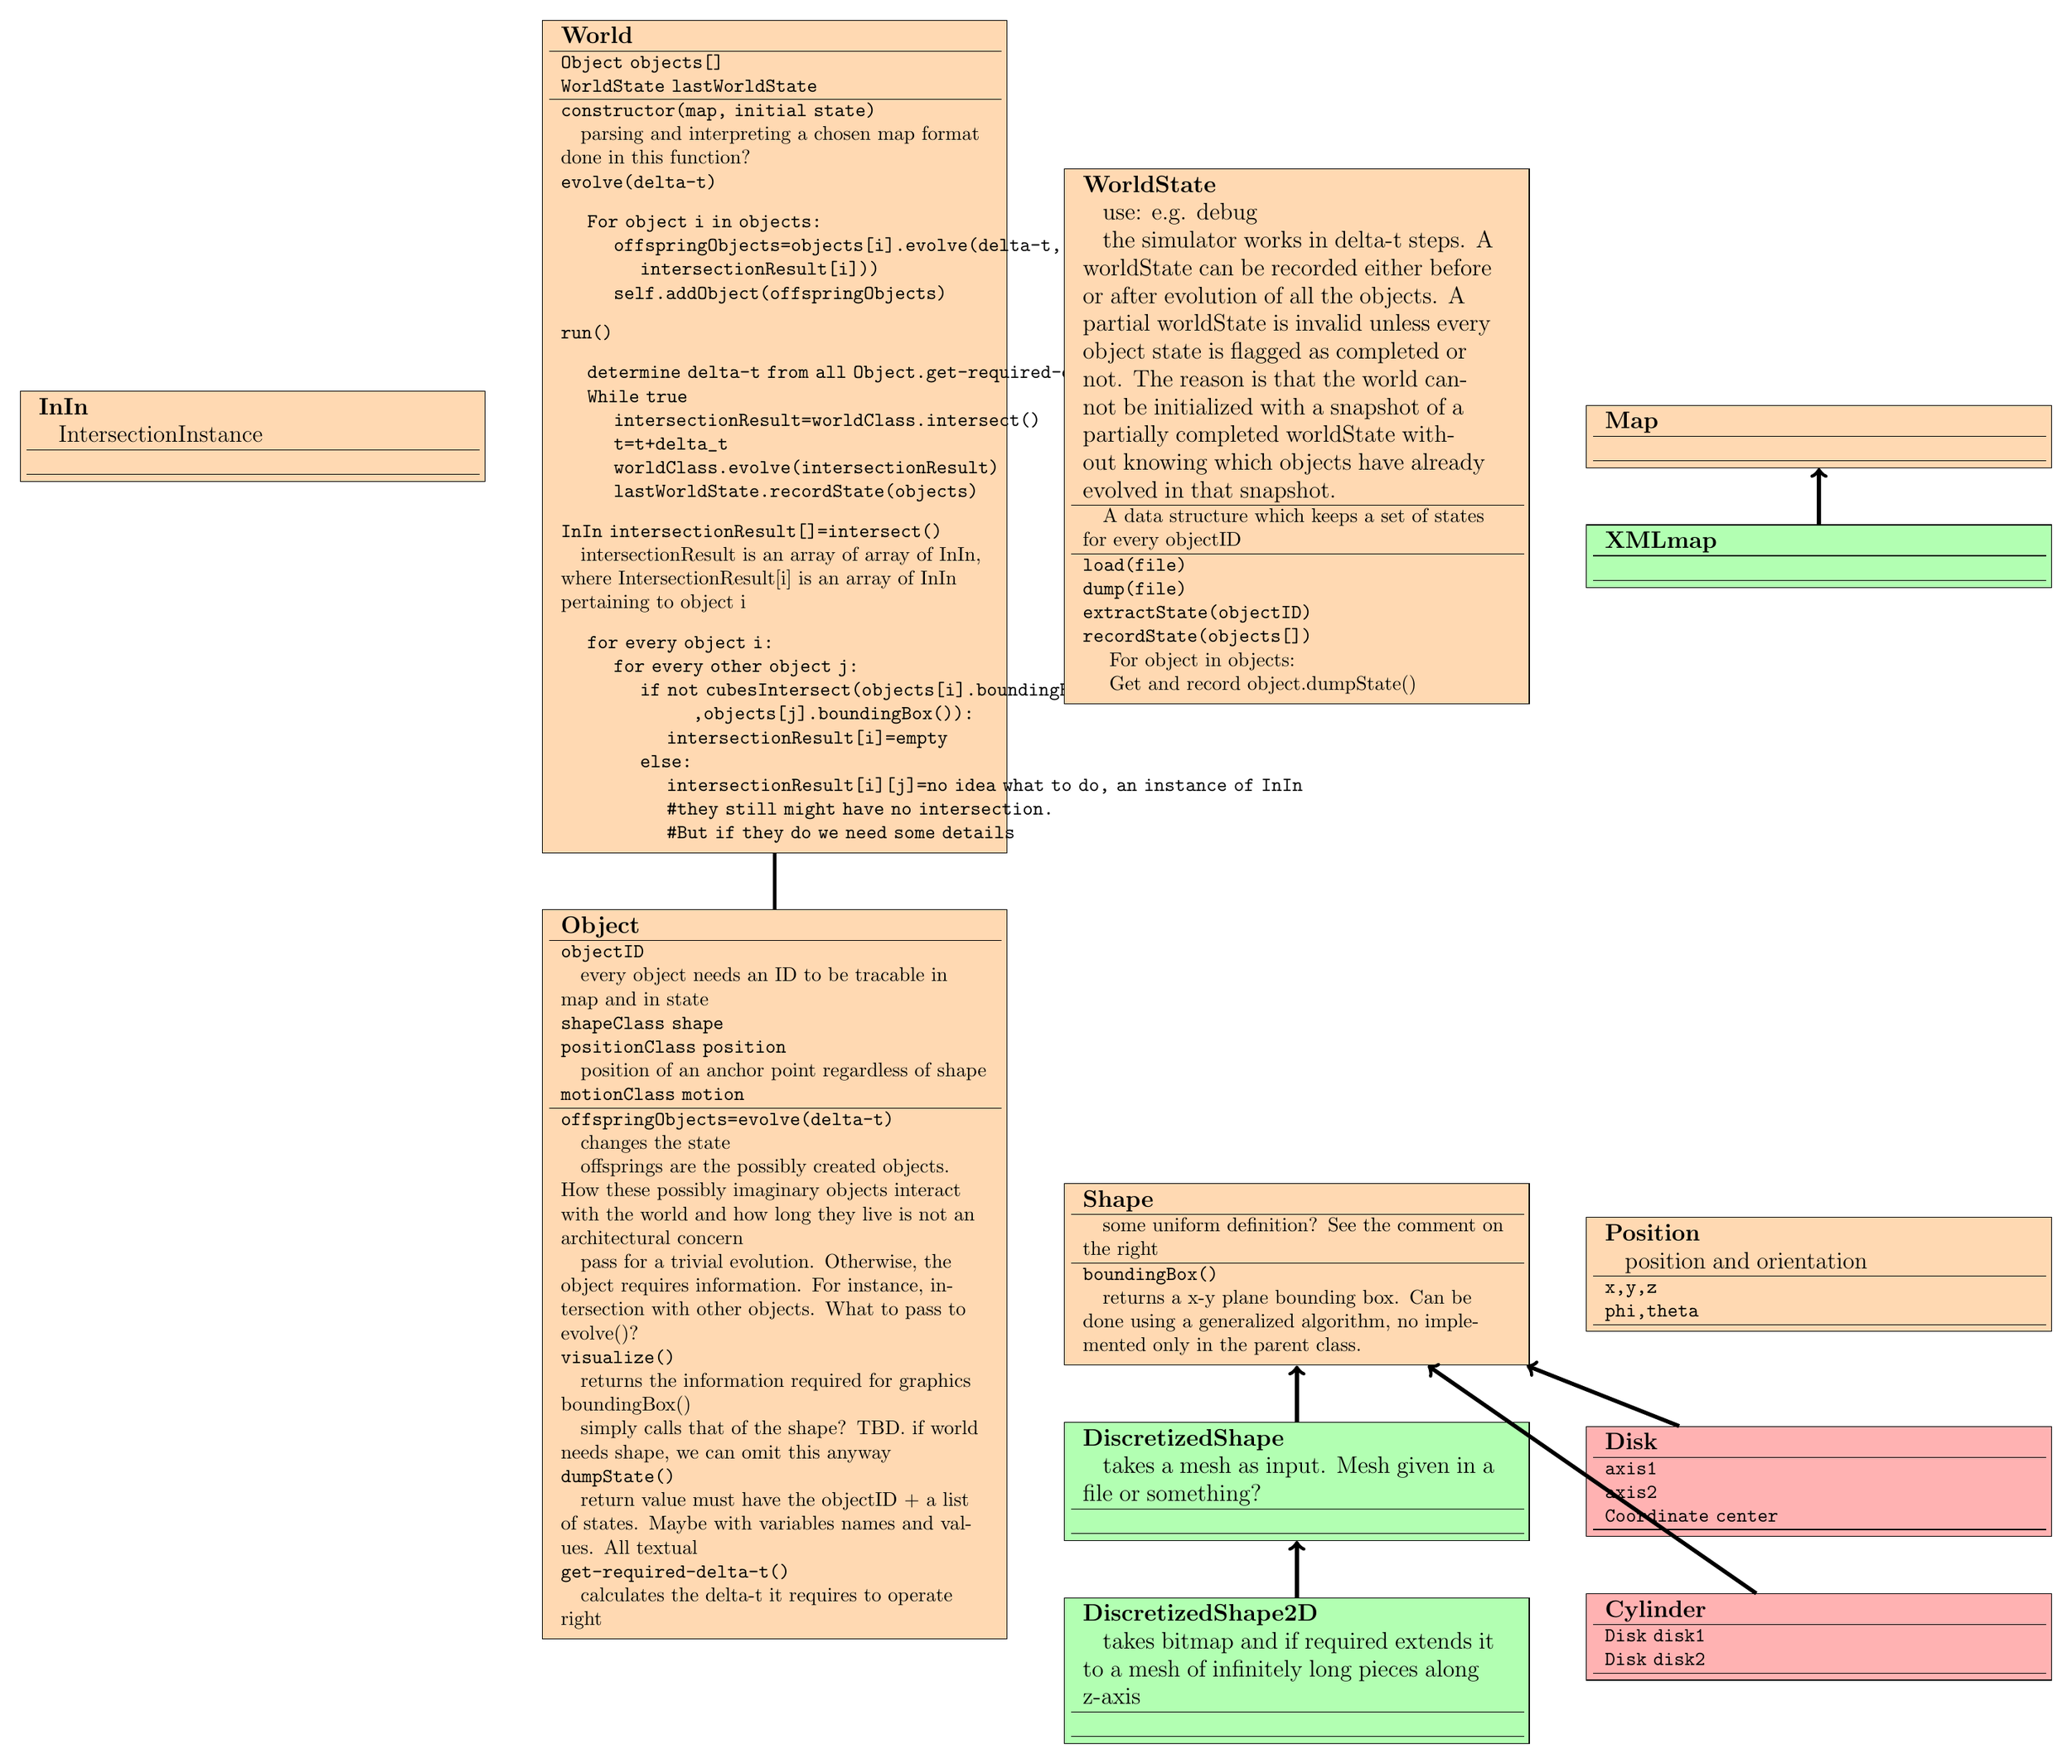
\begin{tikzpicture}


\node[rootClass] (World) {
	\begin{tabular}{p{\nodeTextWidthRatio\textwidth}} 

\className{World}
\\  \hline
\data{Object objects[]}

\data{WorldState lastWorldState}
 \\ \hline 
\method{constructor(map, initial state) }

\desc{parsing and interpreting a chosen map format done in this function?}

\method{evolve(delta-t)}
\begin{verbatim}
    For object i in objects:
        offspringObjects=objects[i].evolve(delta-t, 
            intersectionResult[i]))
        self.addObject(offspringObjects)
\end{verbatim}
\method{run()}
\begin{verbatim}
    determine delta-t from all Object.get-required-delta-t()
    While true
        intersectionResult=worldClass.intersect()
        t=t+delta_t
        worldClass.evolve(intersectionResult)
        lastWorldState.recordState(objects)
\end{verbatim}
\method{InIn intersectionResult[]=intersect()}

\desc{intersectionResult is an array of array of InIn, where IntersectionResult[i] is an array of InIn pertaining to object i}
\begin{verbatim}
    for every object i:
        for every other object j:
            if not cubesIntersect(objects[i].boundingBox()
                    ,objects[j].boundingBox()):
                intersectionResult[i]=empty
            else:
                intersectionResult[i][j]=no idea what to do, an instance of InIn 
                #they still might have no intersection. 
                #But if they do we need some details
\end{verbatim}
\end{tabular} 


};
\node[rootClass,text width=8cm] (Object) [below=of World] {
	\begin{tabular}{p{\nodeTextWidthRatio\textwidth}} 
\className{Object}
\\ \hline
\data{objectID}

\desc{every object needs an ID to be tracable in map and in state}

\data{shapeClass shape}

\data{positionClass position}

\desc{position of an anchor point regardless of shape}

\data{motionClass motion}

\\ \hline
\method{offspringObjects=evolve(delta-t)}

\desc{changes the state}

\desc{offsprings are the possibly created objects. How these possibly imaginary objects interact with the world and how long they live is not an architectural concern}

\desc{pass for a trivial evolution. Otherwise, the object requires  information. For instance, intersection with other objects. What to pass to evolve()?}

\method{visualize()}

\desc{returns the information required for graphics
boundingBox()}

\desc{simply calls that of the shape? TBD. if world needs shape, we can omit this anyway}

\method{dumpState()}

\desc{return value must have the objectID + a list of states. Maybe with variables names and values. All textual}

\method{get-required-delta-t()}

\desc{calculates the delta-t it requires to operate right}

\end{tabular} 


};

\node[rootClass,text width=8cm] (Shape) [right=of Object] {
	\begin{tabular}{p{\nodeTextWidthRatio\textwidth}} 
\className{Shape}
\\ \hline
\desc{some uniform definition? See the comment on the right}
\\ \hline
\method{boundingBox()}

\desc{returns a x-y plane bounding box. Can be done using a generalized algorithm, no implemented only in the parent class.}
\end{tabular} 


};

\node[rootClass,text width=8cm] (Position) [right=of Shape] {
	\begin{tabular}{p{\nodeTextWidthRatio\textwidth}} 
\className{Position}

\desc{position and orientation}
\\  \hline
\data{x,y,z}

\data{phi,theta}
 \\ \hline 
\end{tabular} 


};

\node[rootClass,text width=8cm] (InIn) [left=of World] {
	\begin{tabular}{p{\nodeTextWidthRatio\textwidth}} 
\className{InIn}

\desc{IntersectionInstance}
\\ \hline

\\ \hline
\end{tabular} 


};

\node[rootClass,text width=8cm] (WorldState) [right=of World] {
	\begin{tabular}{p{\nodeTextWidthRatio\textwidth}} 
\className{WorldState}

\desc{use: e.g. debug}

\desc{the simulator works in delta-t steps. A worldState can be recorded either before or after evolution of all the objects. A partial worldState is invalid unless every object state is flagged as completed or not. The reason is that the world cannot be initialized with a snapshot of a partially completed worldState without knowing which objects have already evolved in that snapshot.}
\\  \hline
\desc{A data structure which keeps a set of states for every objectID}
 \\ \hline 
\method{load(file)}

\method{dump(file)}

\method{extractState(objectID)}

\method{recordState(objects[])}

\desc{    For object in objects:}

\desc{         Get and record object.dumpState()}
\end{tabular} 


};

\node[rootClass,text width=8cm] (Map) [right=of WorldState] {
	\begin{tabular}{p{\nodeTextWidthRatio\textwidth}} 
\className{Map}
\\  \hline
 \\ \hline 
\end{tabular} 


};

\draw [instantiatedIn] (Object) -- (World);

\if\showEssentialClasses1
	\node[essentialClass,text width=8cm] (XMLmap) [below=of Map] {
		\begin{tabular}{p{\nodeTextWidthRatio\textwidth}} 
\className{XMLmap}
\\  \hline
 \\ \hline 
\end{tabular} 


	};

	\node[essentialClass,text width=8cm] (DiscretizedShape) [below=of Shape] {
		\begin{tabular}{p{\nodeTextWidthRatio\textwidth}} 
\className{DiscretizedShape}

\desc{takes a mesh as input. Mesh given in a file or something? }
\\ \hline
\\ \hline
\end{tabular} 


	};

	\node[essentialClass,text width=8cm] (DiscretizedShape2D) [below=of DiscretizedShape] {
		\begin{tabular}{p{\nodeTextWidthRatio\textwidth}} 
\className{DiscretizedShape2D}

\desc{takes bitmap and if required extends it to a mesh of infinitely long pieces along z-axis}
\\ \hline
\\ \hline
\end{tabular} 


	};

	\draw [inheritedFrom] (DiscretizedShape) -- (Shape);
	\draw [inheritedFrom] (DiscretizedShape2D) -- (DiscretizedShape);
	\draw [inheritedFrom] (XMLmap) -- (Map);
\fi

\if\showExampleClasses1
	\node[exampleClass,text width=8cm] (Disk) [below=of Shape, right=of DiscretizedShape] {
		\begin{tabular}{p{\nodeTextWidthRatio\textwidth}} 
\className{Disk}
\\ \hline
\data{axis1}

\data{axis2}

\data{Coordinate center}
\\ \hline
\end{tabular} 


	};

	\node[exampleClass,text width=8cm] (Cylinder) [below=of Disk] {
		\begin{tabular}{p{\nodeTextWidthRatio\textwidth}} 
\className{Cylinder}
\\ \hline
\data{Disk disk1}

\data{Disk disk2}

\\ \hline
\end{tabular} 


	};

	\draw [inheritedFrom] (Disk) -- (Shape);
	\draw [inheritedFrom] (Cylinder) -- (Shape);
\fi



%\node[circle, fill=black, below=of filter2, yshift=-0.5cm, inner sep=0pt, minimum width=0.1cm] {};
%\node[circle, fill=black, below=of filter2, yshift=-0.7cm, inner sep=0pt, minimum width=0.1cm] {};
%\node[circle, fill=black, below=of filter2, yshift=-0.9cm, inner sep=0pt, minimum width=0.1cm] {};
%
%\foreach \x/\n in {1/0,2/1,3/N-1}
%	\draw [<-] (filter\x.west) -- +(-0.8cm,0) node [anchor=south] {$A_{\n}$};
%
%\node (adder) [summul,right of=filter2, xshift=2cm, yshift=-1cm] {\Large +};
%
%\foreach \x in {1,2,3}
%	\draw [->] (filter\x.east) -- +(1cm,0) -- (adder);
%
%\draw [->] (adder.east) -- +(0.8cm,0) node [anchor=south] {$s(t)$};
%
%%%%%%%%demodulator
%
%%filter boxes
%\node[block,minimum width=2cm, right=of filter1, xshift=5.5cm] (rfilter1) {$h_0^\ast(-t)$};
%\node[block,minimum width=2cm] (rfilter2) [below=of rfilter1] {$h_1^\ast(-t)$};
%\node[block,minimum width=2cm] (rfilter3) [below=of rfilter2, yshift=-2cm] {$h_{N-1}^\ast(-t)$};
%
%%the three circles
%\node[circle, fill=black, below=of rfilter2, yshift=-0.5cm, inner sep=0pt, minimum width=0.1cm] {};
%\node[circle, fill=black, below=of rfilter2, yshift=-0.7cm, inner sep=0pt, minimum width=0.1cm] {};
%\node[circle, fill=black, below=of rfilter2, yshift=-0.9cm, inner sep=0pt, minimum width=0.1cm] {};
%
%%the sampling block and arrows on both sides and the received symbols
%\foreach \x/\n in {1/0,2/1,3/N-1}
%{
%	\draw [->] (rfilter\x.east) -- +(0.5cm,0) node [anchor=north west] {$T$};
%	\draw (rfilter\x.east) +(0.5cm,0) -- +(0.8cm,0.4cm);
%	\draw [->] (rfilter\x.east) +(0.5cm,0.4) to [bend left=30] +(0.8cm,0cm);
%	\draw (rfilter\x.east) +(0.5cm,0) +(0.8cm,0cm) -- +(1.4cm,0cm) [->] node [anchor=south] {$\hat{A}_{\n}$};
%}
%
%%input signal s(t) with all lines to the filters or multipliers (first filter doesnt have a multiplier)
%\node (input) [left of=rfilter2, xshift=-2cm,yshift=-1cm ] {} ;
%\draw (input) -- +(1cm,0);
%\foreach \x in {1,2,3}
%	\draw (input) +(1cm,0) |- (rfilter\x.west) [->];
%
%%the circles between modulator and demodulator
%\foreach \x in {0.7,0.9,1.1}
%	\node[circle, fill=black, left=of input, xshift=+\x cm, inner sep=0pt, minimum width=0.1cm] {};
	
\end{tikzpicture}

\end{document}
